\chapter{Poisson Processes}
A Poisson process of intensity, or rate, $\lambda > 0$ is an integer-valued stochastic process ${X_t,	t \ge 0}$ for which:
\begin{enumerate}
	\item $X_0 = 0$
	\item For any time points $t_0 = 0 < t_1 < t_2 < s < t_n$, the process increments
	$$X_{t_1}-X_{t_0}, X_{t_2}-X_{t_1}, s, X_{t_n}-X_{t_{n-1}}$$
	are independent random variables, i.e. knowing the number of new arrivals doesn't help to know the next arrivals
	\item For $s \ge 0$ and $t > 0$, the random variable $X_{t+s} - X_s$ has the Poisson distribution
	\begin{equation}\label{p_dist}
		\prob[X_{t+s} - X_s = n] = \frac{(\lambda t)^ne^{-\lambda t}}{n!}
	\end{equation}
	where
	\begin{equation}\label{p_dist_conseq}
		\begin{split}
			\prob[X_n \ge 1] &= \lambda n + o(n) \\
			\prob[X_n \ge 2] &= o(n)
		\end{split}
	\end{equation}
	\gls{kt} at page 226 shows that assuming \eq{p_dist} you can get \eq{p_dist_conseq} and viceversa.
\end{enumerate}
\begin{theorem}[Exponential times in Poisson arrivals]
Interarrival times in a \gls{pp} are iid exponentials with parameter $\lambda$
\end{theorem}
\begin{tikzpicture}
	\begin{axis}[
		y = 1.5cm,
		hide y axis,
		axis x line = bottom,
		xtick={0,1,2,3,4},
		xticklabels={,,$s_0$,$s_1$,$s_2$,$s$}
	]
	\end{axis}
\end{tikzpicture}

\begin{proof}
\begin{equation}
	\prob[S_0 > t] = \prob[\text{No arrivals in } [0,t]] = \frac{(\lambda t)^0 e^{-\lambda t}}{0!} = e^{-\lambda t}
\end{equation}
\begin{equation}\label{poiss_independence}
	\prob[S_1 > t | S_0 = s] = \prob[\text{No arrivals in } [s, s+t]] = \prob[S_1 > t] = e^{-\lambda t}
\end{equation}

Where \eq{poiss_independence} is possible because $S_0$ and $S_1$ are disjoint and so the condition on $S_0$ is independent on the $S_1$ slot.
In general,
\begin{equation}
	\prob[S_n > t | S_i = s_i, ~i=0,s,n-1] = e^{-\lambda t}
\end{equation}
\end{proof}

%LAW OF RARE EVENTS: rare events can be aproximated with a Poisson process? (non ho ben capito)
%REPLY: si dimostra che chiedere eventi rari è equivalente a chiederly Poisson
\section{Properties}

\begin{itemize}
	\item Consider the sum of two independent Poisson process with parameters $\lambda_1$ and $\lambda_2$, what is the outgoing process?
		 \begin{figure}[H]
			\centering
			\begin{tikzpicture}
				 \draw (0,0) circle [radius = 0.5];
			  \draw [->] (-2,1.2) -- (-0.5,0.5);
			  \draw [->] (-2,-1.2) -- (-0.5,-0.5);
			  \draw [->] (0.6, 0) -- (2.6,0);
			  \node at (-1.25, 1.3) {$\lambda_1$};
			  \node at (-1.25, - 1.3) {$\lambda_2$};
			  \node at (1.6 , 0.3) {$\lambda$};
			\end{tikzpicture}
		 \end{figure}
			Given X $\sim Poi(\mu)$, Y $\sim Poi(\nu)$
			\begin{equation}
			 \begin{split}
				  \prob[X + Y = n] &= \sum\limits_{k=0}^n \prob[X = k, Y = n - k] \\
				 &= \sum\limits_{k=0}^n \prob[X = k] \prob[Y = n - k] \\
				 &= \sum\limits_{k=0}^n \frac{e^{-\mu} \mu^k}{k!} \frac{e^{-\nu}\nu^{n-k}}{(n-k)!}\\
				 &= \frac{e^{-(\mu + \nu)}}{n!}\sum\limits_{k=0}^n \frac{n!}{k!(n-k)!}\mu^k\nu^{n-k}\\
				 &= \frac{e^{-(\mu + \nu)}}{n!}(\mu + \nu)^n
			  \end{split}
			 \end{equation}
			 That is Poisson distributed with parameter $\mu + \nu$ (the sum of the two parameters). \\
			 Therefore the outgoing process is Poisson distributed with parameter $\lambda = \lambda_1 + \lambda_2$.
	  \item Now considering the opposite case: two processes generated by the splitting of one (into process $X_1(t)$ with probability $p$ and into process $X_2(t)$ with probability $1-p$)
			 \begin{figure}[H]
					\centering
					 \begin{tikzpicture}
						\draw (0,0) circle [radius = 0.5];
						\draw [->] (0.5, 0.5) -- (2 , 1.2);
						\draw [->] (0.5,-0.5) -- (2, -1.2);
						\draw [->] (-2.6, 0) -- (-0.6, 0);
						\node at (1.25, 1.3) {$\lambda_1$};
						\node at (1.25, - 1.3) {$\lambda_2$};
						\node at (-1.6 , 0.3) {$\lambda$};
						\node at (2.5, 1.2) {$X_1(t)$};
						\node at (2.5, -1.2) {$X_2(t)$};
						\node at (-3.1, 0) {$X(t)$};
					 \end{tikzpicture}
					\end{figure}
			 The resulting processes are independent with parameters $\lambda_1=\lambda p$ and $\lambda_2 = \lambda (1 - p)$.
			 \begin{proof}
				We need to prove that the two processes are Poisson distributed and independent.
				\begin{equation}
				 \begin{split}
					\prob[X_1(t) = n, X_2(t)=m] &= \prob[X_1(t)=n, X(t)= n +m] \\
					&= \prob[X_1(t)=n | X(t)=n+m]\prob[X(t)=n+m]\\
					&= {{n+m}\choose{n}}p^n(1-p)^m \frac{e^{-\lambda t}(\lambda t)^{n+m}}{(n+m)!}\\
					&= \frac{(n+m)!}{n!m!}p^n(1-p)^m e^{-\lambda p t}e^{-\lambda (1-p)t}\frac{(\lambda t)^m (\lambda t)^n}{(n+m)!}\\
					&= \frac{e^{-\lambda p t}(\lambda p t)^n}{n!}\frac{e^{-\lambda (1-p) t}(\lambda (1-p) t)^m}{m!}
				 \end{split}
				\end{equation}
				I can factorize the two distributions and separate them.
							The result are two independent Poisson distributions of parameters $\lambda_1=\lambda p$ and $\lambda_2 = \lambda (1 - p)$.
			 \end{proof}
			 For the result to be proved in general the proof should be done for every possible interval of time. Idea of the proof:
			 \begin{itemize}
				\item disjoint intervals: arrivals already independent $\rightarrow$ trivial
				\item $x_1$ inside $x_2$: I can apply the result I've just proved to $x_1$ first and then to the parts in $x_2$ that are not in $x_1$
				\item $x_1$ and $x_2$ overlapping just on one side: same as before, first apply the previous result to the overlapping part, then to the others
			 \end{itemize}
	\end{itemize}

\section{Distribution related to Poisson Process}
Defining
\begin{itemize}
	\item $X(t)$ as the number of arrivals up to time t;
	\item $W_n$ the instant of $n_{th}$ arrival;
	\item $S_n$= $W_{n+1} - W_n$ the inter-arrival time between $(n+1)_{th}$ and $n_{th}$ arrival;
\end{itemize}

\begin{theorem}[5.4, 	\textbf{$W_n ~ \sim$ Gamma Distribution} ]
	Being $W_{1}$,$W_{2}$,..$W_{n}$ the arrival time in a Poisson Process $N(t)$ with rate ${\lambda}>0$ the probability density function of $W_n$ is the following:

	\begin{equation}
	f_{W_n} (t )=\frac{\lambda^n t^{n-1}} {(n-1)!}e^{-\lambda t} \\
	\end{equation}
\end{theorem}

\begin{theorem}[5.7, Joint probability of [$W_{1}$,..$W_{n}$]]
	Being $W_{1}$,$W_{2}$,..$W_{n}$ the arrival time in a Poisson Process $N(t)$ with rate ${\lambda}>0$. Given $N(t)=n$, the joint distribution of $w_{1}$,$w_{2}$,..$w_{n}$ variables is:
	\begin{equation}
	f_{W_1,W_2,..W_n|n} (w_1,w_2,..w_n) = P (W_1=w_1,...W_n=w_n|N(t)=n) = n!/t^n
	\end{equation}
	\begin{proof}
		Excluding simultaneous arrivals,
		\begin{equation*}
			\begin{cases}
				P[N(t+h)-N(t)=0]= 1 - \lambda h+ o(h) \\
				P[N(t+h)-N(t)=1]= \lambda h+ o(h) \\
				P[N(t+h)-N(t)>=0]= o(h) \text{, negligible as } h\rightarrow 0
			\end{cases}
		\end{equation*}

		The event $ \{w_i<W_i \leq w_i+\Delta w \}$ for $i=1,...,n$ and $N(t)=n$ correspond to the following events:
		\begin{equation*}
			\begin{cases}
				E_1=\{\text{0 arrivals out of } \Delta w_i \} \\
				E_2=\{\text{1 arrival in each of } \Delta w_i \}
			\end{cases}
		\end{equation*}

		Compute the probability of these two disjoint events.
		\begin{equation}
			\begin{split}
				& P[N((0,w_1])=0,...,N((w_n+\Delta w_n,t])=0] = \\
				& = e^{-\lambda w_1} e^{-\lambda (w_2-(w_2+\Delta w_2))} ... e^{-\lambda (t-(w_n+\Delta w_n))} \\
				& =e^{-\lambda t} (1+o(max\{\Delta w_i\}))
			\end{split}
		\end{equation}
		\begin{equation}
			\begin{split}
				P[N((w_1,,w_1+\Delta w_1]) &=1,...,N((w_n,w_n+\Delta w])=1] =\\
				& = (\lambda \Delta w_1) ... (\lambda \Delta w_n) (1+o(\max\{\Delta w_i\}))
			\end{split}
		\end{equation}

		So, the final probability is computed as the product of probability of these two independent events:
		\begin{equation}
			\begin{split}
				& f_{W_1,W_2,..W_n|n} (w_1,w_2,..w_n)( \Delta w_1\Delta w_2..\Delta w_n) = \\
				& =P[E_1 \cap E_2 ]\\
				& =P[w_i\leq W_i \leq w_i+\Delta w_i, i=1,2,..,n| \textnormal{n arrivals}]=\\
				& =\frac{P[w_i\leq W_i \leq w_i+\Delta w_i, i=1,2,..,n,\textnormal{n arrivals}}{\textnormal{n arrivals}}\\
				& =\frac{(\lambda \Delta w_1 e^{-\lambda w_1}..\lambda \Delta w_n e^{-\lambda w_n})e^{-\lambda t}}{\frac{(\lambda t)^{n}e^{-\lambda t}} {n!}}\\
				& =\frac{ (\Delta w_1 \Delta w_2.. \Delta w_n) n!}{t^n}
			\end{split}
		\end{equation}

		Dividing both members for ($\Delta w_1 \Delta w_2 .. \Delta w_n$) we obtain the distribution of an uniform random variable.
		\begin{equation}
			f_{W_1,W_2,..W_n|n} (w_1,w_2,..w_n) =n!/t^n
		\end{equation}
	\end{proof}
\end{theorem}

\begin{theorem}[5.5,\textbf{Exponential Inter-arrival} ]
	The Inter-arrival times $S_0,S_1, S_{n-1}$ are independent exponential r.v.
	\begin{equation}
		f_{S_k}(s)=\lambda e^{-\lambda s}, s \ge 0
	\end{equation}
\end{theorem}

\begin{theorem}[5.6, Conditioned Arrivals]
	(Enunciate given in an intuitive but not so formal way)

	Being $X(t)$ a Poisson Process with $\lambda>0$, $u$ and $t$ two temporal variables such that $0<u<t$, $n$ and $k$ two variables which describes the number of arrivals such that $0\leq k\leq n$ . The probability of the event "up to instant $u$, $k$ arrivals have been occurred conditioned by the fact that $n$ arrivals occurs up to time $t$" is described by a binomial distribution with $n$ attempts and $u/t$ success probability.

	Formally
	\begin{equation}
		P[X(u)=k|X(t)=n]= \frac{n!}{k!(n-k)!}\bigg(\frac{u}{t}\bigg)^k\bigg(1-\frac{u}{t}\bigg)^{n-k}
	\end{equation}
\end{theorem}

\begin{proof}
	It is a direct consequence of Theorem 5.7.
	Being $X(t)=n$, the position of each arrival along interval $t$ can be modeled as i.i.d. uniform random variable. This corresponds to the realization of n experiments with $p_{succ}=u/t$ thus the conditioned probability can be modeled as binomial $Bin(n,\frac{u}{t})$.
\end{proof}

\section{M/G/$\infty$}

\begin{figure}[h]
	\centering
	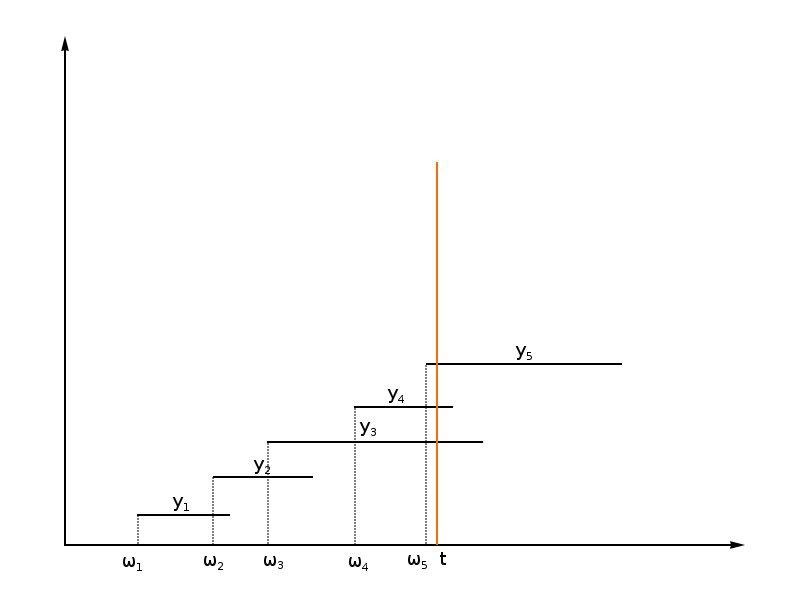
\includegraphics[width=0.8\textwidth]{img/mginf}
	\caption{Representation of a system with Poisson distributed arrivals}
\end{figure}

For the M/G/$\infty$ queue, we define these special quantities, in order to build an associate \gls{mc}.
\begin{equation*}
	\begin{cases}
		X(t) = \text{ number of arrivals in }[ 0, t ] \\
		M(t) = \text{ number of users in the system at time }t
	\end{cases}
\end{equation*}

A user is still in the system at time $t$ if $W_k + Y_k \geq t$. Therefore $M(t) = \sum\limits_{k=1}^{X(t)} \mathds{1}\{W_k + Y_k \geq t\} $.
\begin{equation}
	\begin{split}
		\prob[M(t)=m|X(t)=n] &= \prob\bigg[\sum\limits_{k=1}^{X(t)} \mathds{1}\{W_k + Y_k \geq t\} = m|X(t)=n\bigg] \\
		&= \prob\bigg[\sum\limits_{k=1}^{n} \mathds{1}\{U_k + Y_k \geq t\}\bigg] = {{n}\choose{m}}p^{m}(1-p)^{n-m}
	\end{split}
\end{equation}

Where $p = \prob[U_k + Y_k \geq t]$, we have to compute this probability.
\begin{equation}
	\begin{split}
	 p = \prob[U_k + Y_k \geq t] &= \frac{1}{t}\int_0^t \prob[Y_k \geq t -u] \mathrm{d}u \\
	 &= \frac{1}{t}\int_0^t [1 - G(t-u)] \mathrm{d}u
	 &= \frac{1}{t}\int_0^t [1 - G(z)] \mathrm{d}z
	\end{split}
\end{equation}

Now we can compute
\begin{equation}
	\begin{split}
		\prob[M(t)=m] &= \sum\limits_{n=0}^{\infty} \prob[M(t)=m|X(t)=n]\prob[X(t)=n] \\
		&= \sum\limits_{n=m}^{\infty} \frac{n!}{m!(n-m)!}p^m(1-p)^{n-m}\frac{e^{-\lambda t} (\lambda t)^n}{n!} \\
		&= \frac{e^{-\lambda t} (\lambda p t)^m}{m!}\sum\limits_{n=m}^{\infty} \frac{(1-p)^{n-m}(\lambda t)^{n-m}}{(n-m)!}\\
		&= \frac{e^{-\lambda t} (\lambda p t)^m}{m!} e^{-\lambda(1-p)t}\\
		&= \frac{e^{-\lambda p t}(\lambda p t)^m}{m!}
	\end{split}
\end{equation}
Where $\lambda p t = E[M(t)] = \lambda t \frac{1}{t} \int_0^t [1 - G(z)] \mathrm{d}z = \lambda \int_0^t [1 - G(z)] \mathrm{d}z$. \\
As $t \rightarrow \infty$: $\lambda \int_0^t [1 - G(z)] \mathrm{d}z = \lambda E[Y]$ where $1/\lambda$ is the average interarrival time, and $E[Y]$ is the average service time.

%shot noise example? should we add it?

\section{BG 275: Slotted multi-access}
Assumptions:
\begin{enumerate}
	\item Slotted system: constant packet duration, synchronized users
	\item Poisson arrivals: with \textbf{total} arrival rate $\lambda$
	\item Collision or perfect reception
	\item Immediate $ \{ 0,1, e\}$ feedback, where 0 stands for \textit{no packets arrived}, 1 stands for \textit{one packet arrived} and \textit{e} stands for \textit{too many packets arrived}, i.e. \textit{collision}.
	\item Retransmission until success (backlogged)
	\item No buffering $\rightarrow$ upper bound to the performance of a realistic system
	\item Infinite set of nodes $\rightarrow$ lower bound
\end{itemize}
The last two assumptions provide a system with $n$ packets in it and $n$ nodes ready to process them (each node receives 1 packet).
In a real system, a node may have more than 1 packet.

\subsection{ALOHA}
\begin{equation*}
	\begin{cases}
		\text{Slot time }= 1 \\
		G = \text{ average number of attempts per slot} \\
		S = \text{ average number of successes per slot} \\
		\lambda = \text{ average rate of arrivals (new packet per slot)} \\
	\end{cases}
\end{equation*}

The success probability is $P_{succ} = e^{-T G} = e^{-2 G}$, as the vulnerability interval is $T=2$.
Now suppose to consider the interval $d\tau$, we have
\begin{equation}\begin{split}
	\text{A stationary process:} \\
	\begin{cases}
		\prob[\text{one TX starts in $d\tau$}] &\approx G d\tau\\
		\exp[\text{number of successes in $d\tau$}] &= G e^{-2 G} d\tau \\
	\end{cases}
	\end{split}
	\end{equation}
	\begin{equation}\begin{split}
	\exp\bigg[\text{number of successes in $[0;t]$}\bigg] &= \int\limits_0^t G e^{-2 G}d\tau = t G e^{-2 G}\\
	\text{S = throughput }&=\frac{1}{t} \int\limits_0^t G e^{-2 G}d\tau = G e^{-2 G}\\
	\implies S_{max} = \frac{1}{2e}& \approx 18.7\% \quad G_{max} = \frac{1}{2}
\end{split}\end{equation}

If the user transmits only at the end of the (universal) time: Slotted ALOHA.
With SA the vulnerability interval becomes T=1. $\implies S_{max}=\frac{1}{e} \approx 37\% \quad G_{max} = 1$.

Actually, this analysis can not be completely correct, since we suppose G as fixed in order to find a working point. In a real system, G cannot be fixed. In the follows we propose an approach to take in account this problem.

\subsubsection{Correct approach}

Suppose $m$ users.

Let the state of the system be n, which considers the number of backlogged users.
The traffic per user is $\frac{\lambda}{m}$ and let the probability that a backlogged user transmits in a slot be $q_r$. Suppose the retransmission probability density function be a geometric, then a non-backlogged user transmits with probability $q_a = 1-e^{-\frac{\lambda}{m}}$.

As the arrival are Poissonian and the retransmission are memoryless, we can study this case with \gls{mc}.

\begin{equation}\begin{split}
	Q_a(i,n) &= \prob[\text{i new arrivals per TX | state n}] = \binom{m-n}{i} q_a^i (1-q_a)^{m-n-i} \\
	Q_r(i,n) &= \prob[\text{i ReTX | state n}] = \binom{n}{i} q_r^i (1-q_r)^{n-i} \\
\end{split}\end{equation}
Now we want to define the transition probability $P_{n,n+1}$, and the calculations provide the following cases:
\begin{equation}
	P_{n,n+1} = \begin{cases}
	 Q_a(i,n) & 2 \le i \le m-n \\
	 Q_a(1,n) [1-Q_r(0,n)] & i=1 \quad \text{1 arrival, no departures}\\\\
	 \begin{aligned}
	 & Q_a(0,n) [1-Q_r(1,n)] + \\ & Q_a(1,n) Q_r(0,n)
	 \end{aligned}& i=0 \quad \parbox[t]{0.6\textwidth}{no arrivals, 1 departure (successful reTX) or 1 arrival successfully transmitted }\\\\
	 Q_a(0,n) Q_r(1,n) & i = -1 \quad \text{1 departure, no arrivals}\\
	 0 & i < -1 \quad \text{no more than one departure}
	\end{cases}
\end{equation}
We can conclude that the resulting matrix is an almost-upper-triangular.

\subsubsection{Drift Analysis}
\begin{equation}
	\begin{split}
		D_n &= \exp[\text{change in state} | n] = \exp[X_{t+1} - X_t | X_t = n] \\
		&= \exp[\text{arrivals - departures} | n ] = (m-n) q_a - P_{succ} \\
		P_{succ}&= \prob[\text{exactly 1 TX}|n] = Q_a(1,n) Q_r(0,n) + Q_a(0,n) Q_r(1,n) \\
		&= (m-n)(1-q_a)^{n-m-1} q_a (1-q_r)^n + (1-q_a)^{m-n} n q_r (1-q_r)^{n-1} \\
		&= (1-q_a)^{m-n} (1-q_r)^n \bigg[\frac{m-n}{1-q_a} q_a + \frac{n q_r}{1-q_r}\bigg]
	\end{split}
\end{equation}
we can then approximate $(1+x)^n \approx e^{-n x}$ if $x \ll 1$
\begin{equation}
	\implies P_{succ} \approx e^{-(m-n) q_a} e^{-n q_r} \overbrace{[(m-n) q_a + n q_r]}^{G(n)}
	\implies P_{succ} \approx G(n)e^{-G(n)}
\end{equation}

We found out that the success probability depends on the state, so we would like to know how the states evolve in time.
The process can be approximated as a Poisson Process and the description is given by $D_n = (m-n) q_a - G(n) e^{-G(n)}$
with G(n) as given before.

\begin{figure}
	\centering
	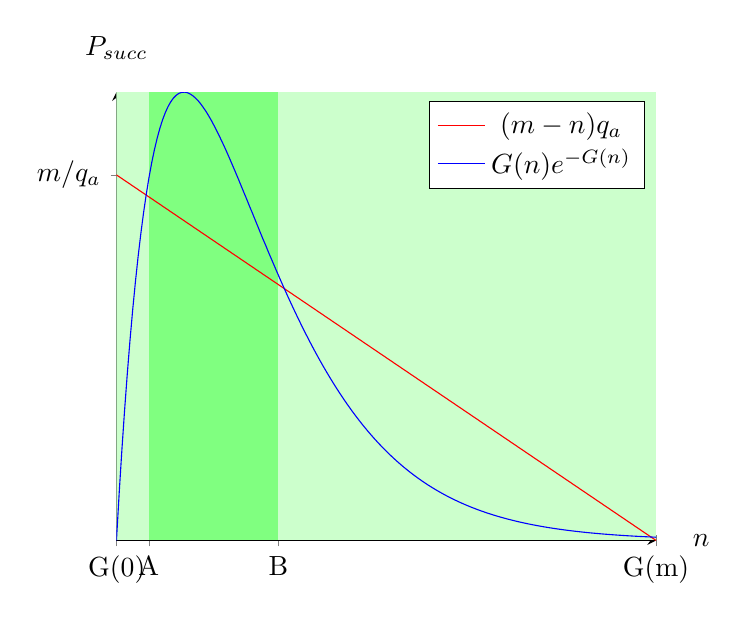
\begin{tikzpicture}
\begin{axis}[axis lines=middle,samples=200
        ,ylabel=$P_{succ}$
        ,xlabel=$n$
        ,every axis x label/.style={
          at={(ticklabel* cs:1.05)},
            anchor=west,
          },
        every axis y label/.style={
          at={(ticklabel* cs:1.05)},
            anchor=south,
          },
        ,xtick=data,
        ,xtick={0.001,0.12,0.6,2}
        ,xticklabels={G(0),A, B,G(m)}
        ,ytick=data,
        ,ytick={0.3}
        ,yticklabels={$m/q_a$}
        ]
			\fill[green!20]
				(axis cs:0,0) --
				(axis cs:0.12,0) --
				(axis cs:0.12,2) --
				(axis cs:0,2) --
				cycle;
			\fill[green!50]
				(axis cs:0.12,0) --
				(axis cs:0.6,0) --
				(axis cs:0.6,2) --
				(axis cs:0.12,2) --
				cycle;
			\fill[green!20]
				(axis cs:0.6,0) --
				(axis cs:2,0) --
				(axis cs:2,2) --
				(axis cs:0.6,2) --
				cycle;
      \addplot[red,domain=0:2] {0.15*(2-x)};
      \addplot[blue,domain=0:2] {4*x*e^(-4*x)};
			\addlegendentry{$(m-n)q_a$}
			\addlegendentry{$G(n)e^{-G(n)}$}
    \end{axis}\end{tikzpicture}

	\caption{Between \textbf{A} and \textbf{B} and for any G(n) bigger than \textbf{G(m)} $D_n <0$. $D_n>0$ in the other regions of the plane}
	\label{fig:drift}
\end{figure}

When $D_n>0$ the system tends to reduce the backlogging, wherease if $D_n<0$ the backlogging increases and the system becomes unstable. The optimal condition for the system is $D_n = 0$, when this condition is verified, the system is in an equilibrium point.

We would like to improve the system, such that the probability of the system to become
unstable, is small and the delay to be as low as possible; to do so we can:
\begin{description}
	\item[increase $q_r$] The delay gets smaller, but the stability get worse
	\item[decrease $q_r$] the delay increases, but the system is more stable
\end{description}

Considering the limit, when $m \to +\infty$, $q_a \to 0 \implies q_a \approx \frac{\lambda}{m}$
As $G=\lambda + n q_r$ we'd like to maximize the throughput and the success probability.
$G_{max}=1 = \lambda + n  q_r \implies q_r = \frac{1-\lambda}{n} \implies q_r = q_r(n)$

We don't know n, so we need to extimate $q_r(n)$ to best fit. We will call the maximized G version
of ALOHA as the \emph{Stabilized Aloha}.

\begin{lemma}[Pakes' lemma (B.G. p.264)]

	Given $D_i = \exp[X_{n+1}-X_n|X_n = 1]$ the drift, suppose $D_i < +\infty ~\forall i$ and that $\exists \delta > 0 , ~i_0$ index s.t.
	$D_i \le - \delta ~\forall i > i_0$ ($D_i$ is bounded away from zero)\\
	Then the \gls{mc} is \emph{stable} (or positive recurrent).

\end{lemma}
\begin{proof}
	Since the drift is bounded, we can always find a maximum values in some interval.
 Let $\beta = \max_{i \le i_0} D_i$ . Then $\forall i$:
 \begin{equation}\begin{split}
	\exp[X_n | X_0 = i] -i &= \sum\limits_{k=1}^n \exp[X_k - X_{k-1}|X_0 = i] \\
	&= \sum\limits_{k=1}^n \sum\limits_{j=0}^{+\infty} \exp[X_k - X_{k-1}|X_{k-1} = j , X_0 = i ] P_{i,j}^{(k-1)}\\
	& \le \sum\limits_{k=1}^{n} \left[\beta \sum\limits_{j=0}^{i_0} P_{i,j}^{(k-1)} - \delta (1- \sum\limits_{j=0}^{i_0} P_{i,j}^{(k-1)}\right]\\
	&= (\beta + \delta) \sum\limits_{k=1}^n \sum\limits_{j=0}^{i_0} P_{i,j}^{(k-1)} - n \delta \\
	\implies & 0 \le \exp[X_n | X_0 = i] \le (\beta + \delta) \sum\limits_{k=1}^n \sum\limits_{j=0}^{i_0} P_{i,j}^{(k-1)} - n \delta +i\\
	& \quad \text{as it's valid $\forall n , i$ we can say that} \\
	\exp[X_n | X_0 = i] &= n \left[(\beta + \delta) \sum\limits_{j=0}^{i_0} \frac{1}{n} \sum\limits_{k=1}^{n} P_{i,j}^{(k-1)} - \delta \right] +i\\
	\text{As $n \to +\infty$ } & \text{ we can write}\\
	0 \le \lim_{n \to +\infty} &\bigg[(\beta + \delta) \sum\limits_{j=0}^{i_0} \underbrace {\frac{1}{n} \sum\limits_{k=1}^{n} P_{i,j}^{(k-1)}}_{\pi_j} - \delta + \underbrace{\frac{i}{n}}_{\to 0}\bigg]\\
	0 \le &\underbrace{(\beta + \delta)}_{>0} \sum\limits_{j=0}^{i_0} \pi_j - \delta \quad \text{\textbf{CONTRADDICTION }if } \pi_j = 0 ~\forall j \\
	\implies & \text{it must be positive recurrent}
	\end{split}\end{equation}
\end{proof}

\begin{lemma}[Kaplan's lemma]
Suppose that $\exists i_0 ~and ~k \text{ s.t. } D_i>0 ~\forall i> i_0 , \; P_{i,j} = 0 ~\forall i,j \; 0 \le j \le i-k$
Then the \gls{mc} is unstable (i.e. non-positive recurrent)

\begin{figure}
	\centering
	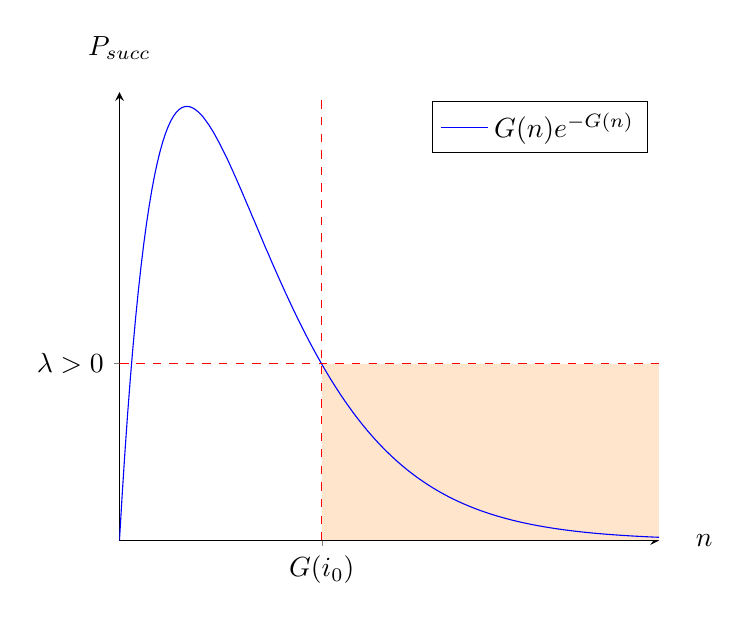
\begin{tikzpicture}
\begin{axis}[axis lines=middle,samples=200
        ,ylabel=$P_{succ}$
        ,xlabel=$n$
        ,every axis x label/.style={
          at={(ticklabel* cs:1.05)},
            anchor=west,
          },
        every axis y label/.style={
          at={(ticklabel* cs:1.05)},
            anchor=south,
          },
        ,xtick=data,
        ,xtick={0.75}
        ,xticklabels={$G(i_0)$}
        ,ytick=data,
        ,ytick={0.15}
        ,yticklabels={$\lambda>0$}
        ]
			\fill[orange!20]
				(axis cs:0.75,0) --
				(axis cs:2,0) --
				(axis cs:2,0.15) --
				(axis cs:0.75,0.15) --
				cycle;
			\addplot[blue,domain=0:2] {4*x*e^(-4*x)};
      \addplot[red,domain=0:2, dashed] {0.15};
			\addplot[red,domain=0:2, dashed] coordinates {(0.75,0) (0.75,0.38)};
			\addlegendentry{$G(n)e^{-G(n)}$}
    \end{axis}\end{tikzpicture}

	\caption{In the orange region, the function is unstable, in according to the Kaplan's Lemma.}
	\label{fig:kaplan}
\end{figure}

We may want the \gls{mc} to be stable at least for an amount of time (i.e. network can fail once or twice a year).
\end{lemma}

Slotted Aloha exploits at max $S \approx 37 \%$ of its maximum throughput, so we'd like to reduce the wasted time,
so that we can increase $S \to 100\%$. To do so, we need
\begin{enumerate}
	\item Coordination
	\item See if the channel is empty and determine what's happening (\textbf{CSMA})
\end{enumerate}

Let $\beta = \frac{\tau}{L/C} = \frac{\tau C}{L}$. If $\beta \ll 1 \; \implies \text{CSMA is effective}$. \\
L.A.N are defined by $\beta \ll 1$.

If user generates a packet in an empty time slot, he will try to send it in the next slot. If the packet is generated while the channel is in use, the packet will be backlogged.

State transitions take $\begin{cases}
	\beta & \text{if empty slot} \\
	\beta + 1 & \text{if there's a transmission}
\end{cases}$

\begin{equation}\begin{split}
	\prob[\text{empty slot }|n] &= e^{-\lambda \beta} (1-q_r)^n \\
	\exp[\text{slot duration}] &= \beta + 1 - e^{-\lambda\beta} (1-q_r)^n \\
	D_n &= \exp[\text{arrivals - departures }|n ]= \lambda [\beta + 1 - e^{-\lambda \beta} (1-q_r)^n ]\\
	P_{succ} &= \lambda \beta e^{-\lambda \beta} (1-q_r)^n + e^{-\lambda \beta} (1-q_r)^{n-1} n q_r \\
	&\approx (\lambda \beta + n q_r) e^{-(\lambda \beta + n q_r)} \quad \text{ if } n q_r \ll 1 \\
	&= g(n) e^{g(n)}
\end{split}\end{equation}

\begin{figure} \centering
	\begin{tikzpicture}\begin{axis}[axis lines=middle,samples=200
        ,ylabel=$P_{succ}$
        ,xlabel=$S$
        ,ymax=1
        ,every axis x label/.style={
          at={(ticklabel* cs:1.05)},
            anchor=west,
          },
        every axis y label/.style={
          at={(ticklabel* cs:1.05)},
            anchor=south,
          },
        ,xtick=data
        ,xtick={0.98}
        ,xticklabels={$\frac{1}{1+\sqrt{2\cdot \beta}}$}
        ,ytick=data,
        ,ytick={0.3748,0.748}
        ,yticklabels={$\lambda$,$\frac{1}{1+\sqrt{2\cdot \beta}}$}
        ]
      \addplot[red,domain=0:6] {2*x*e^(-x)};
      \addplot[blue,domain=0:6] {x*e^(-x)};
      \addplot[gray,dotted,domain=0:6] {0.3748};
      \addplot[gray,dotted,domain=0:6] {0.748};
      \addplot[gray,dotted,mark=none] coordinates {(0.98, 0) (0.98, 3)};
    \end{axis}\end{tikzpicture}

	\caption{The new system, in red, perform always better than Aloha, in blue}
	\label{}
\end{figure}
If two transmissions occours at the same tume, but the nodes transmitting are far enough, they won't hear each other and packets will collide.

\begin{table}[h!]
	\centering
	\begin{tabular}{|c|c|c|}
		\textbf{Type} & \textbf{Duration} & \textbf{Probability} \\ \hline
		IDLE & $\beta$ & $e^{-\lambda \beta} (1-q_r)^n \approx e^{-g(n)}$ \\
		SUCCESS & $1+\beta$ & $\approx g(n) e^{-g(n)}$ \\
		COLLISION & $2 \beta$ & $1-(1+g(n)) e^{-g(n)}$
	\end{tabular}
	\caption{Events occouring in the CSMA channel}
	\label{TAB:tx_prob}
\end{table}
$D_n \lessgtr 0 $ if $\lambda \lessgtr \frac{g(n) e^{-g(n)}}{\beta + 1 - e^{-g(n)}}$\\
We know that instability will occour eventually, but the time for it to happen is really long.

\subsection{Recurrent \gls{mc} behaviour}
Suppose a recurrent \gls{mc} like the one in figure \ref{fig:recurrMC}, we can study a system which has a transient state and two states, 0 and 1,
that may be recurrent.
\begin{figure}[h!]\centering
	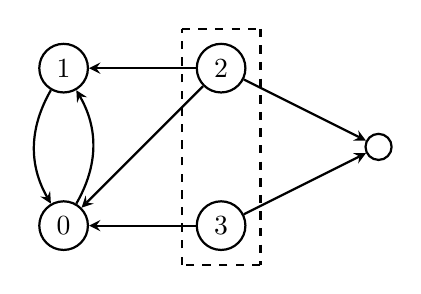
\begin{tikzpicture}
      [auto, thick,
  blk/.style={rectangle , draw=black , thick ,rounded corners,
  minimum height =2 em, align=center,text width=1.55cm, text=black,
   text opacity=1},
  nodeChain/.style={circle,draw=black, thick,minimum size=0.1cm,
  fill opacity=0.2,draw opacity=1, text=black,text opacity=1, align=center}
  ]
  \node[nodeChain] at (-2,-1) (zero) {0};
  \node[nodeChain] at (-2,1) (one) {1};
  \node[nodeChain] at (0,1) (two) {2};
  \node[nodeChain] at (0,-1) (three) {3};
  \node[nodeChain] at (2,0) (four){};
  \draw[-stealth] (zero) to[bend right]  (one);
  \draw[-stealth] (one) to[bend right]  (zero);
  \draw[-stealth] (two) -- (one);
  \draw[-stealth] (two) --  (zero);
  \draw[-stealth] (three) -- (zero);
  \draw[-stealth] (two) -- (four);
  \draw[-stealth] (three) -- (four);
  \draw[dashed] (-0.5,1.5) -- (0.5,1.5);
  \draw[dashed] (0.5,1.5)-- (0.5,-1.5);
  \draw[dashed]  (-0.5,-1.5) -- (-0.5,1.5);
  \draw[dashed]  (0.5,-1.5) -- (-0.5,-1.5);
\end{tikzpicture}

	\caption{ State 0 and 1 form a periodic class, state 2 and 3 are the transient
	and the state on the right represent the other possible states in that markov chain}
	\label{fig:recurrMC}
\end{figure}

\begin{equation}\begin{split}
	P&=\begin{pmatrix}
		Q & R_1 & R_2 \\
		0 & A  & 0 \\
		0 & 0  & 1 \\
	\end{pmatrix}\\
	\text{where, }&\forall n\ge 0
	A^{2n+1}&=\begin{pmatrix}
		0 & 1 \\
		1 & 0 \\
	\end{pmatrix}\\
	A^{2n}&=\begin{pmatrix}
		1 & 0 \\
		0 & 1 \\
	\end{pmatrix}\\
\end{split}\end{equation}

We than have that

\begin{equation}\begin{split}
	P^2&=\begin{pmatrix}
		Q^2 & Q R_1 + R_1 A & Q R_2 + R_2\\
		0 & A^2  & 0 \\
		0 & 0  & 1 \\
	\end{pmatrix}
	\\
	P^{3} = P P^2 &=\begin{pmatrix}
		Q^3 & Q^2 Q R_1 A + R_1 A^2 & Q^2 R_2 + Q R_2 +R_2\\
		0 & A^3=A  & 0 \\
		0 & 0  & 1 \\
	\end{pmatrix}\\
	P^{n+1}&=\begin{pmatrix}
		Q^{n+1} & \sum\limits_{i=0}^n Q^i R_1 A^{n-i} & \sum\limits_{i=0}^n Q^i R_2\\
		0 & A^{n+1}  & 0 \\
		0 & 0  & 1 \\
	\end{pmatrix}\\
\end{split}\end{equation}
We can now evaluate separately the case where n is even and the one where it's odd

\begin{equation}\begin{split}
	n &= 2 k \\
	&\sum\limits_{i=0}^{2k}Q^i R_1 A^{2k-i} = \sum\limits_{j=0}^{k}Q^{2j} R_1 + \sum\limits_{j=0}^{k-1}Q^{2j+1} R_1 A \\
	&=\left(\sum\limits_{j=0}^{k}Q^{2j} \right) R_1 + \left(\sum\limits_{j=0}^{k-1}Q^{2j} \right) (Q R_1 A)\\
	\implies & k \to +\infty \quad [I - Q^2]^{-1} (R_1 + Q R_1 A)\\
	n &= 2 k + 1 \\
	&\sum\limits_{i=0}^{2k+1}Q^i R_1 A^{2k+1-i} = \sum\limits_{j=0}^{k}Q^{2j} R_1 A + \sum\limits_{j=0}^{k}Q^{2j+1} R_1 \\
	\implies & k \to +\infty \quad [I - Q^2]^{-1} (R_1 A + Q R_1 ) \\
	\\
	&\text{the two limits are the same if: }\\
	& [I - Q^2]^{-1} (R_1 + Q R_1 A) = [I - Q^2]^{-1} (R_1 A + Q R_1 )\\
	\implies & det(1-Q^2)\neq 0\\
	& [I-Q ] R_1 = [I-Q] R_1 A \quad \implies R_1 = R_1 A
\end{split}\end{equation}


\subsection{PASTA property (Poisson Arrivals See Time Averages)}
\begin{equation}
	\prob[N(t)=n|A(t,t+\delta)] = \prob[N(t)=n]
\end{equation}
At time $t$ I have $n$ users, so $N(t)=n$ depends on past, wherease $A(t,t+\delta)$ depends on the future.

Under mild\footnote{Mild as a feather, not as a salsa.} conditions:
\begin{enumerate}
	\item the system is stable
	\item the system state changes in unit increments
\end{enumerate}
If the chain is stable, the state n will be visited an infinite numer of times. In particular, the arrivals and the departures can be written as:
\begin{equation}\begin{split}
a_n(t)&= \frac{\text{\# of arrivals finding n}}{\text{\# of arrivals}} = \frac{\text{\# of transitions } n \to n+1}{\text{\# of upwards transitions}}\\
d_n(t)&= \frac{\text{\# of departures leaving n}}{\text{\# of departures}} = \frac{\text{\# of transitions } n+1 \to n}{\text{\# of downwards transitions}}
\end{split}\end{equation}
